%%%%%%%%%%%%%%%%%%%%%%%%%%%%%%%%%%%%%%%%%%%%%%%%%%%%%%%%%%%%%%%%%%%%%%%%
\clearpage
\section{Sheared and deformed objects}

\section{Non-equilibrium static form factor of a reptating chain}
\begin{figure}[htb]
\begin{center}
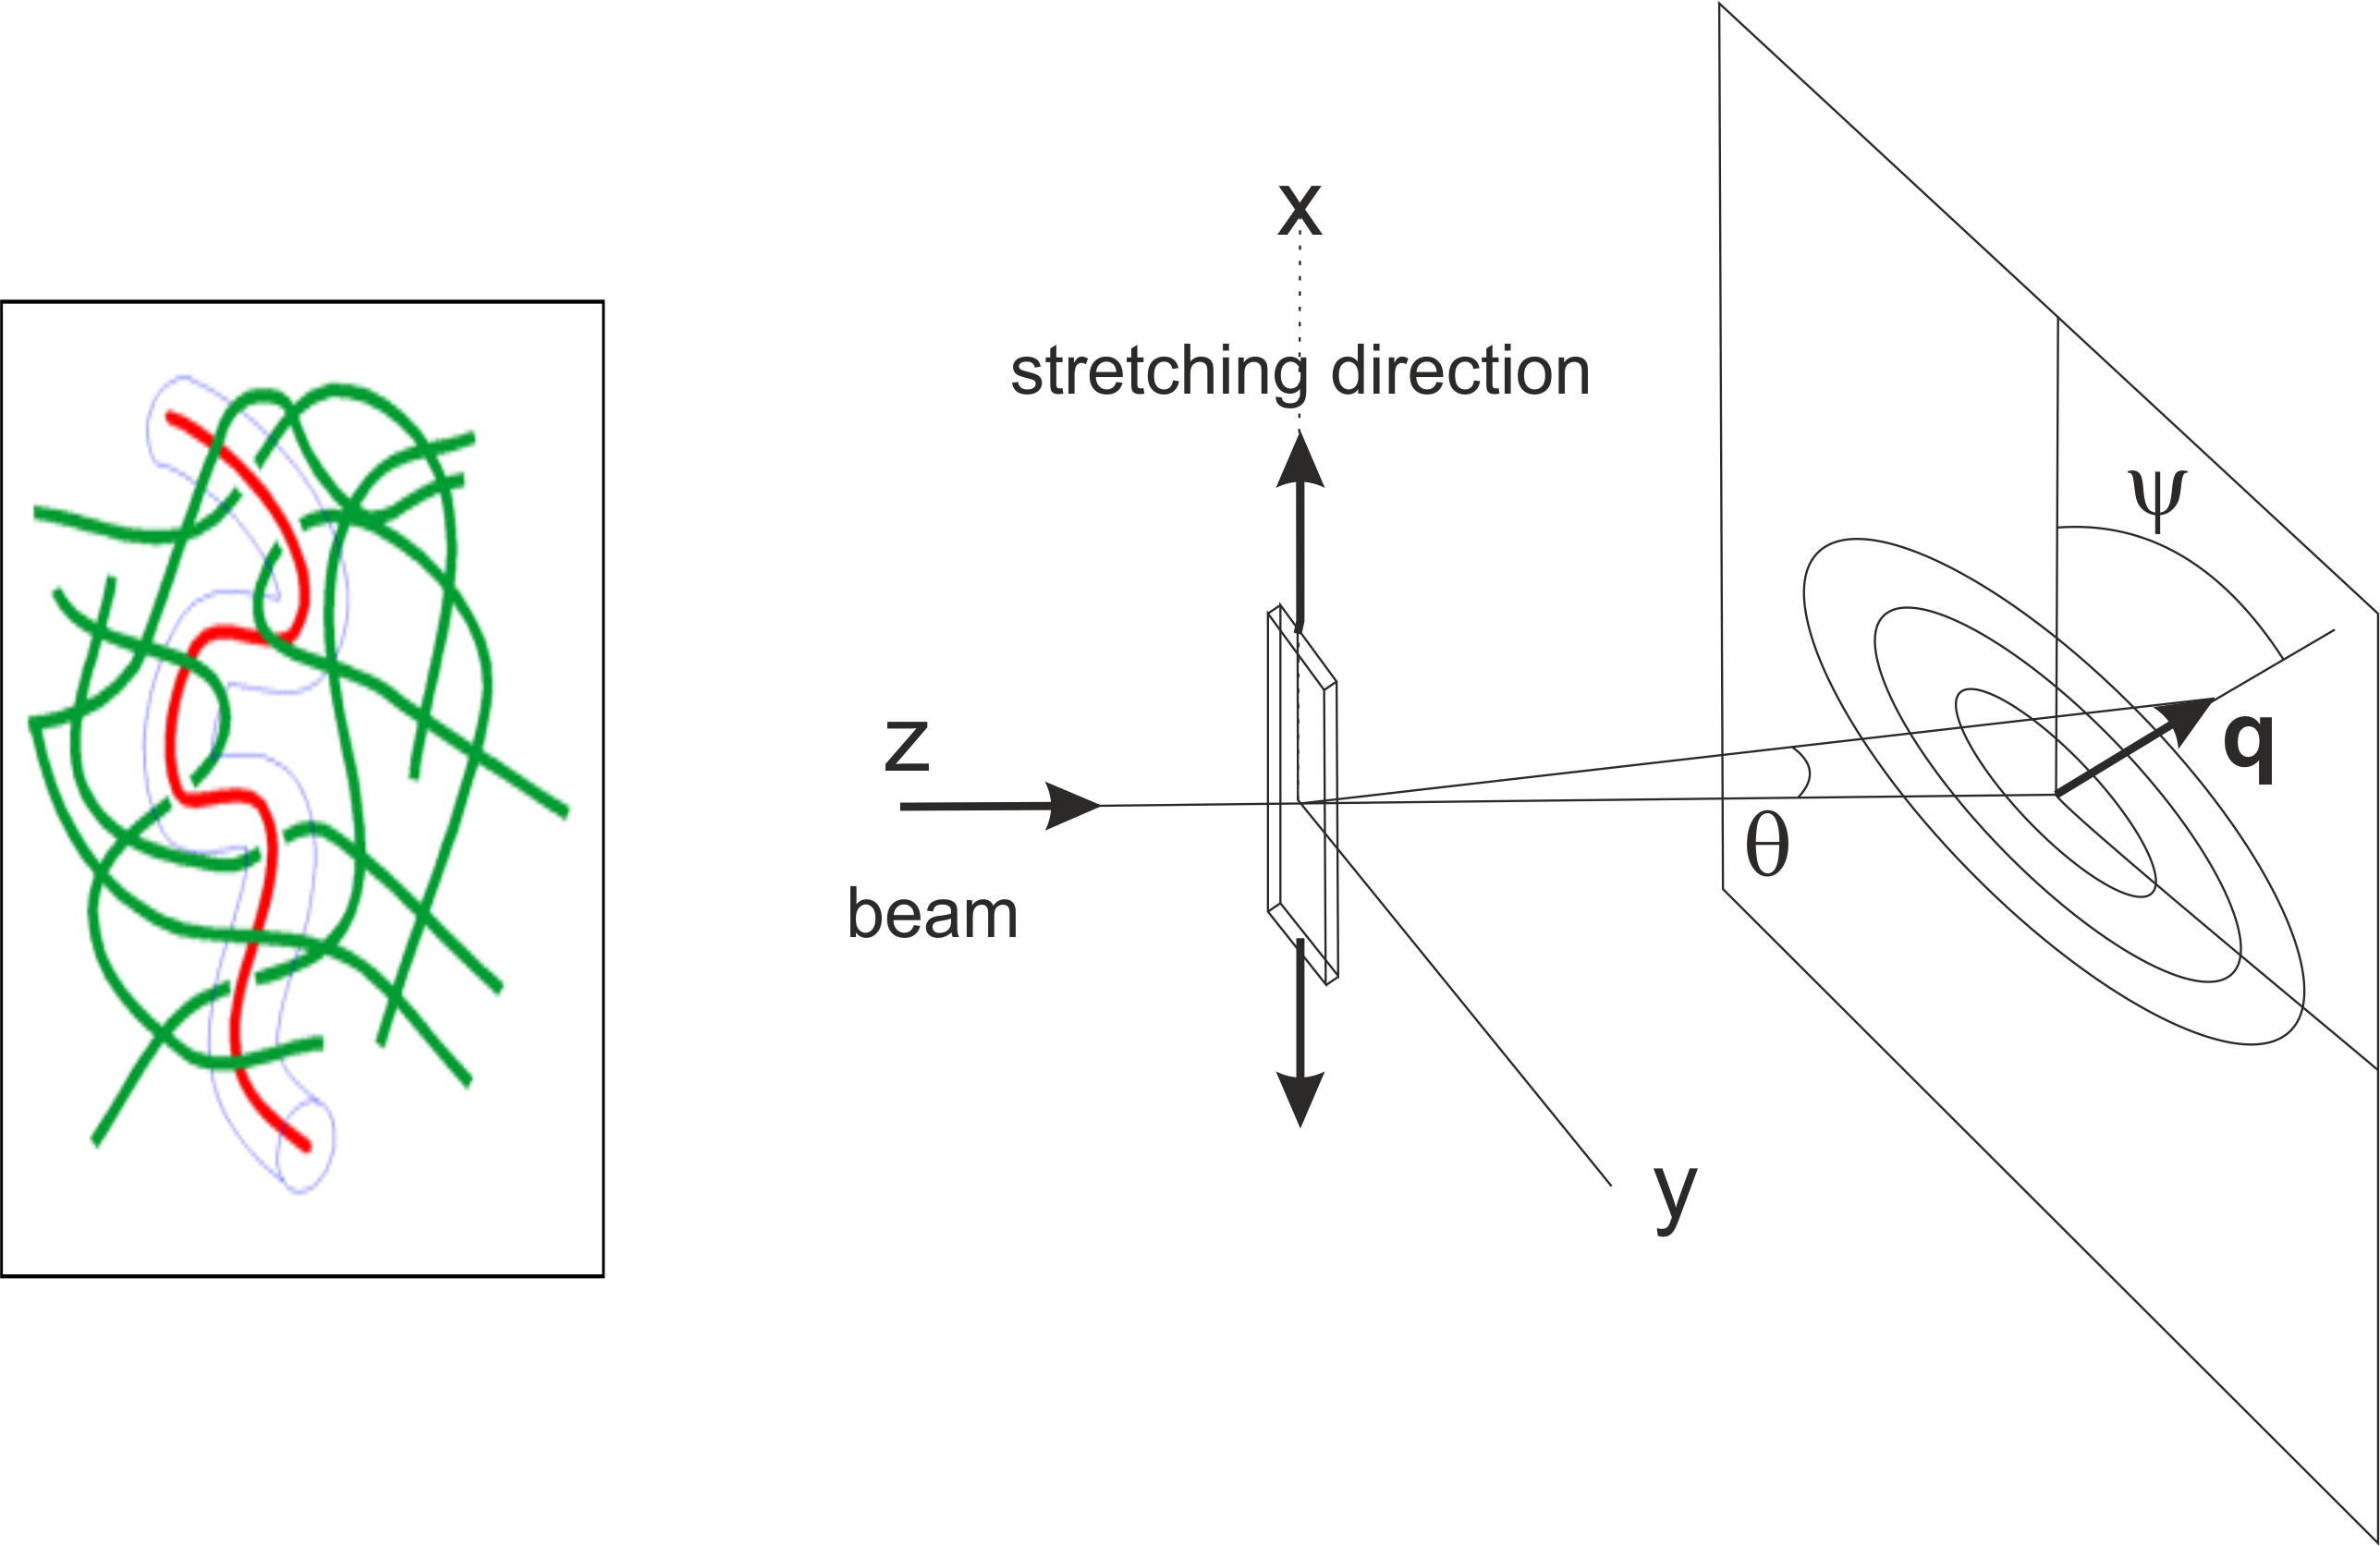
\includegraphics[width=\textwidth]{../images/form_factor/reptating_chain/reptating_chain.png}
\end{center}
\caption{Sketch of experimental setup for stretching a polymer melt.}
\label{fig:stretchpolymermelt}
\end{figure}
This model \cite{Hong1983,Noolandi1984} describes the scattering behaviour of an uniaxial deformed (stretched) Gaussian polymer chain as a function of the deformation ratio and Rouse relaxation time. The model might not include an up-to-date tube model but shows some main features of deformed polymer melts.
\begin{align}
\begin{split}
I\left(q,\frac{t}{\tau}\right)/I_0 = & \hspace{\breite}
                                        D(\alpha) + \frac{1}{6}(\alpha-\beta) \left(1+e^{-\alpha}\right) H\left(\alpha,\frac{t}{\tau}\right) \\
                                     & + \frac{1}{6}(\alpha-\beta)^2 e^{-\beta} \int_0^1 \mathrm{d}y \, y^3 e^{\beta y} \left(1+e^{-\alpha y}\right) H\left(\alpha y,\frac{t}{\tau y^2}\right)
\end{split}
\end{align}
with
\begin{align}
H\left(x,\frac{t}{\tau}\right) &= \frac{96}{\pi^2} \sum_{n = \mathrm{odd}} \frac{1}{n^2\left(n^2\pi^2+x^2\right)} e^{-n^2 \frac{t}{\tau}}
\end{align}
$D(x)$ is the Debye function $D(x) = 2\left(x - 1 + e^{-x}\right)/x^2$, $\alpha = q^2 R_g^2$, $R_g$ is the equilibrium radius of gyration
of the chain and $\tau$ is the reptation time or tube disengagement time.
Furthermore $\lambda$ is the uniaxial elongation factor, $q_\parallel$ and $q_\perp$ are respectively the components of the wave vector $q$ in directions parallel and
perpendicular to the direction of elongation which than define the parameter $\beta$ as
\begin{align}
\beta &= \left(q_\parallel^2\lambda^2+q_\perp^2/\lambda\right) R_g^2/E \\
E &= \frac{1}{2} \left\{\lambda +\frac{\mathrm{asinh}\left(\sqrt{\lambda^3-1}\right)}{\sqrt{\lambda\left(\lambda^3-1\right)}} \right\} \\
q_\parallel &= q \cos(\psi-\theta_0) \\
q_\perp &= q \sin(\psi-\theta_0)
\end{align}

\hspace{1pt}\\
\underline{Input Parameters for models \texttt{CylShell1}, \texttt{CylShell2} and \texttt{LongCylShell}:}\\
\begin{description}
\item[\texttt{I0}] forward scattering $I_0$
\item[\texttt{Rg}] radius of gyration of unstretched polymer $R_r$
\item[\texttt{lambda}] stretching factor $\lambda$
\item[\texttt{t/tau}] relaxation time in units of Rouse time $t/\tau$
\item[\texttt{theta\_0}] stretching direction in the detector plane $\theta_0$ in degree
\item[\texttt{psi}] $\mathbf{q}$-direction $\psi$ in the detector plane in degree
\end{description}

\underline{Note:}
\begin{itemize}
\item The model only converges for $\lambda >1$.
\end{itemize}

\begin{figure}[htb]
\begin{center}
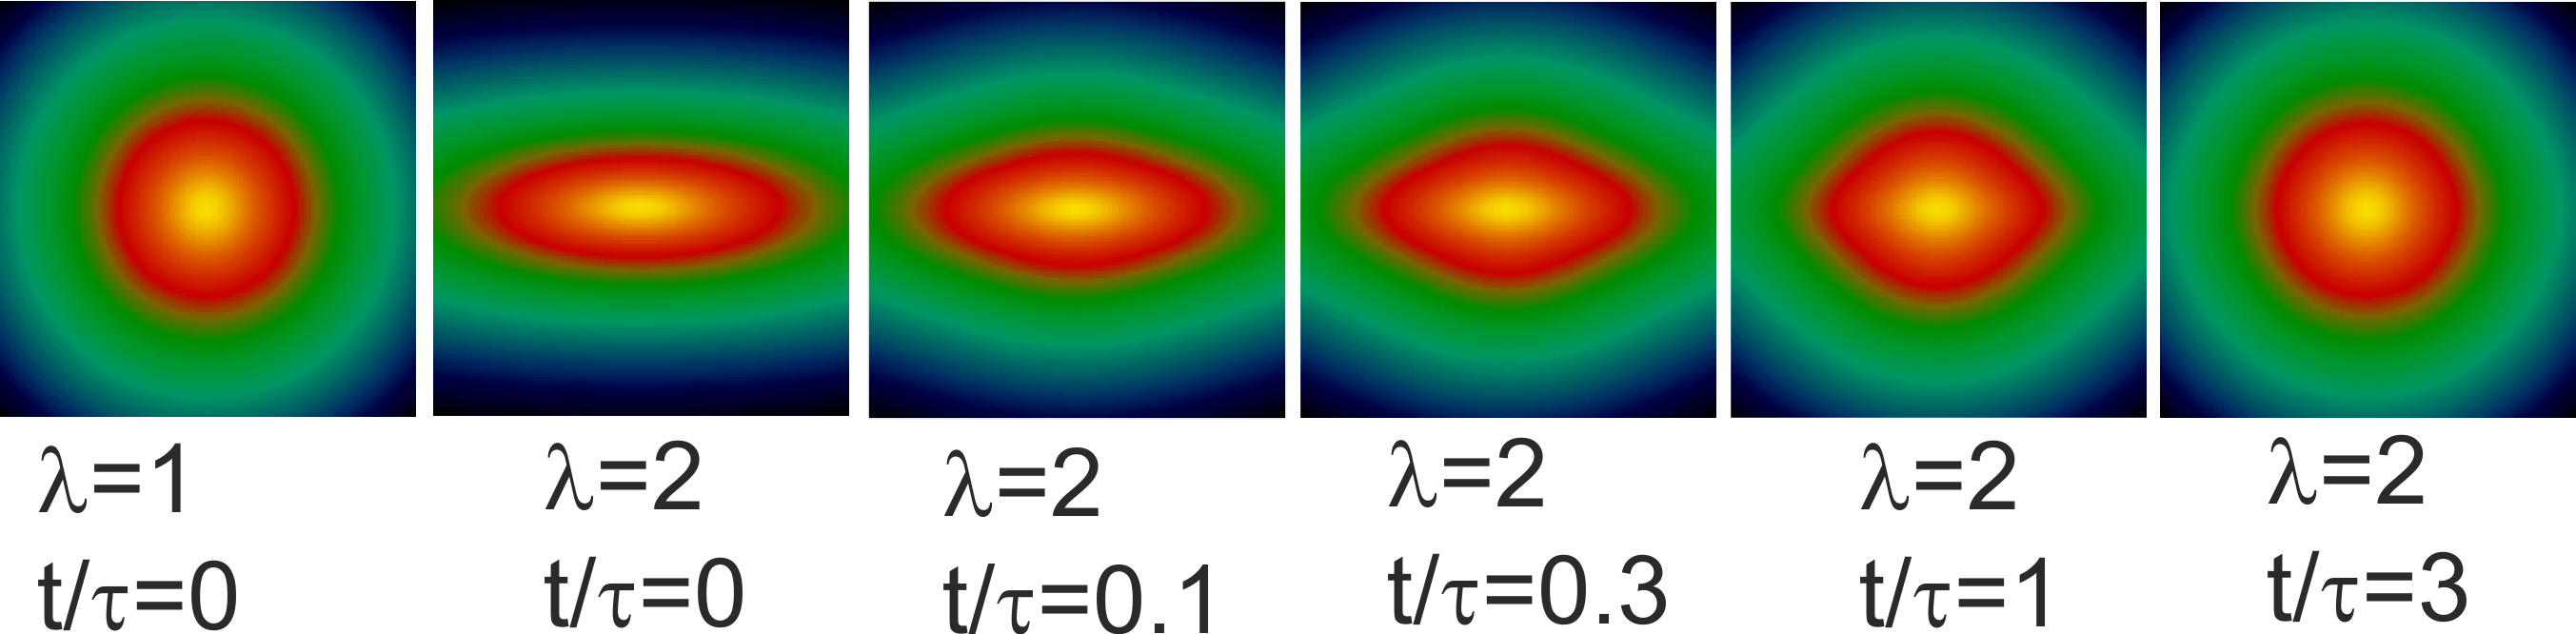
\includegraphics[width=\textwidth]{../images/form_factor/reptating_chain/lambda_2_reptating_chains.png}
\end{center}
\caption{2D scattering patterns for different relaxation times $t/\tau$ after a deformation step of $\lambda=2$}
\label{fig:IQ2Dstretchedpolymermelt}
\end{figure}

%%%%%%%%%%%%%%%%%%%%%%%%%%%%%%%%%%%%%%%%%%%%%%%%%%%%%%%%%%%%%%%%%%%%%%%%%

\subsection{ShearedCylinderHayterPenfold \cite{Hayter1984}}
\label{sect:ShearedCylinderHayterPenfold}
\hspace{1pt}\\

\begin{figure}[htb]
\begin{center}
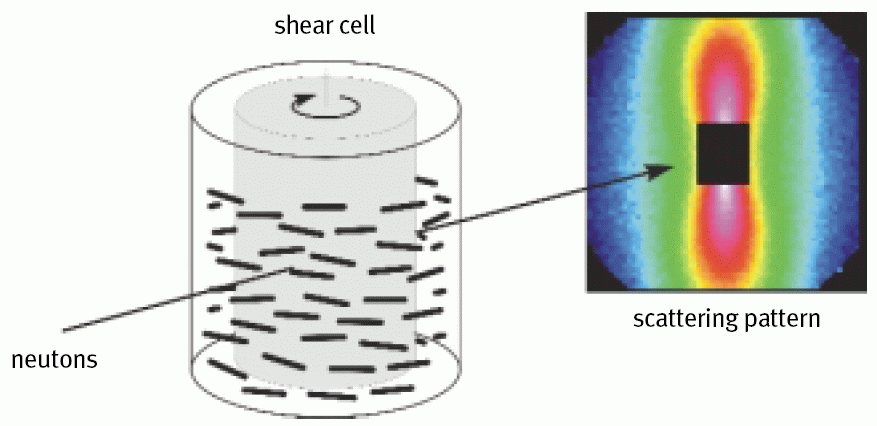
\includegraphics[width=0.7\textwidth,height=0.3\textwidth]{sheared_cylinders1.png}
\end{center}
\caption{Shear orientation of micelles in a shear cell with the
corresponding SANS-pattern.} \label{sheared_cylinders1}
\end{figure}

\begin{figure}[htb]
\begin{center}
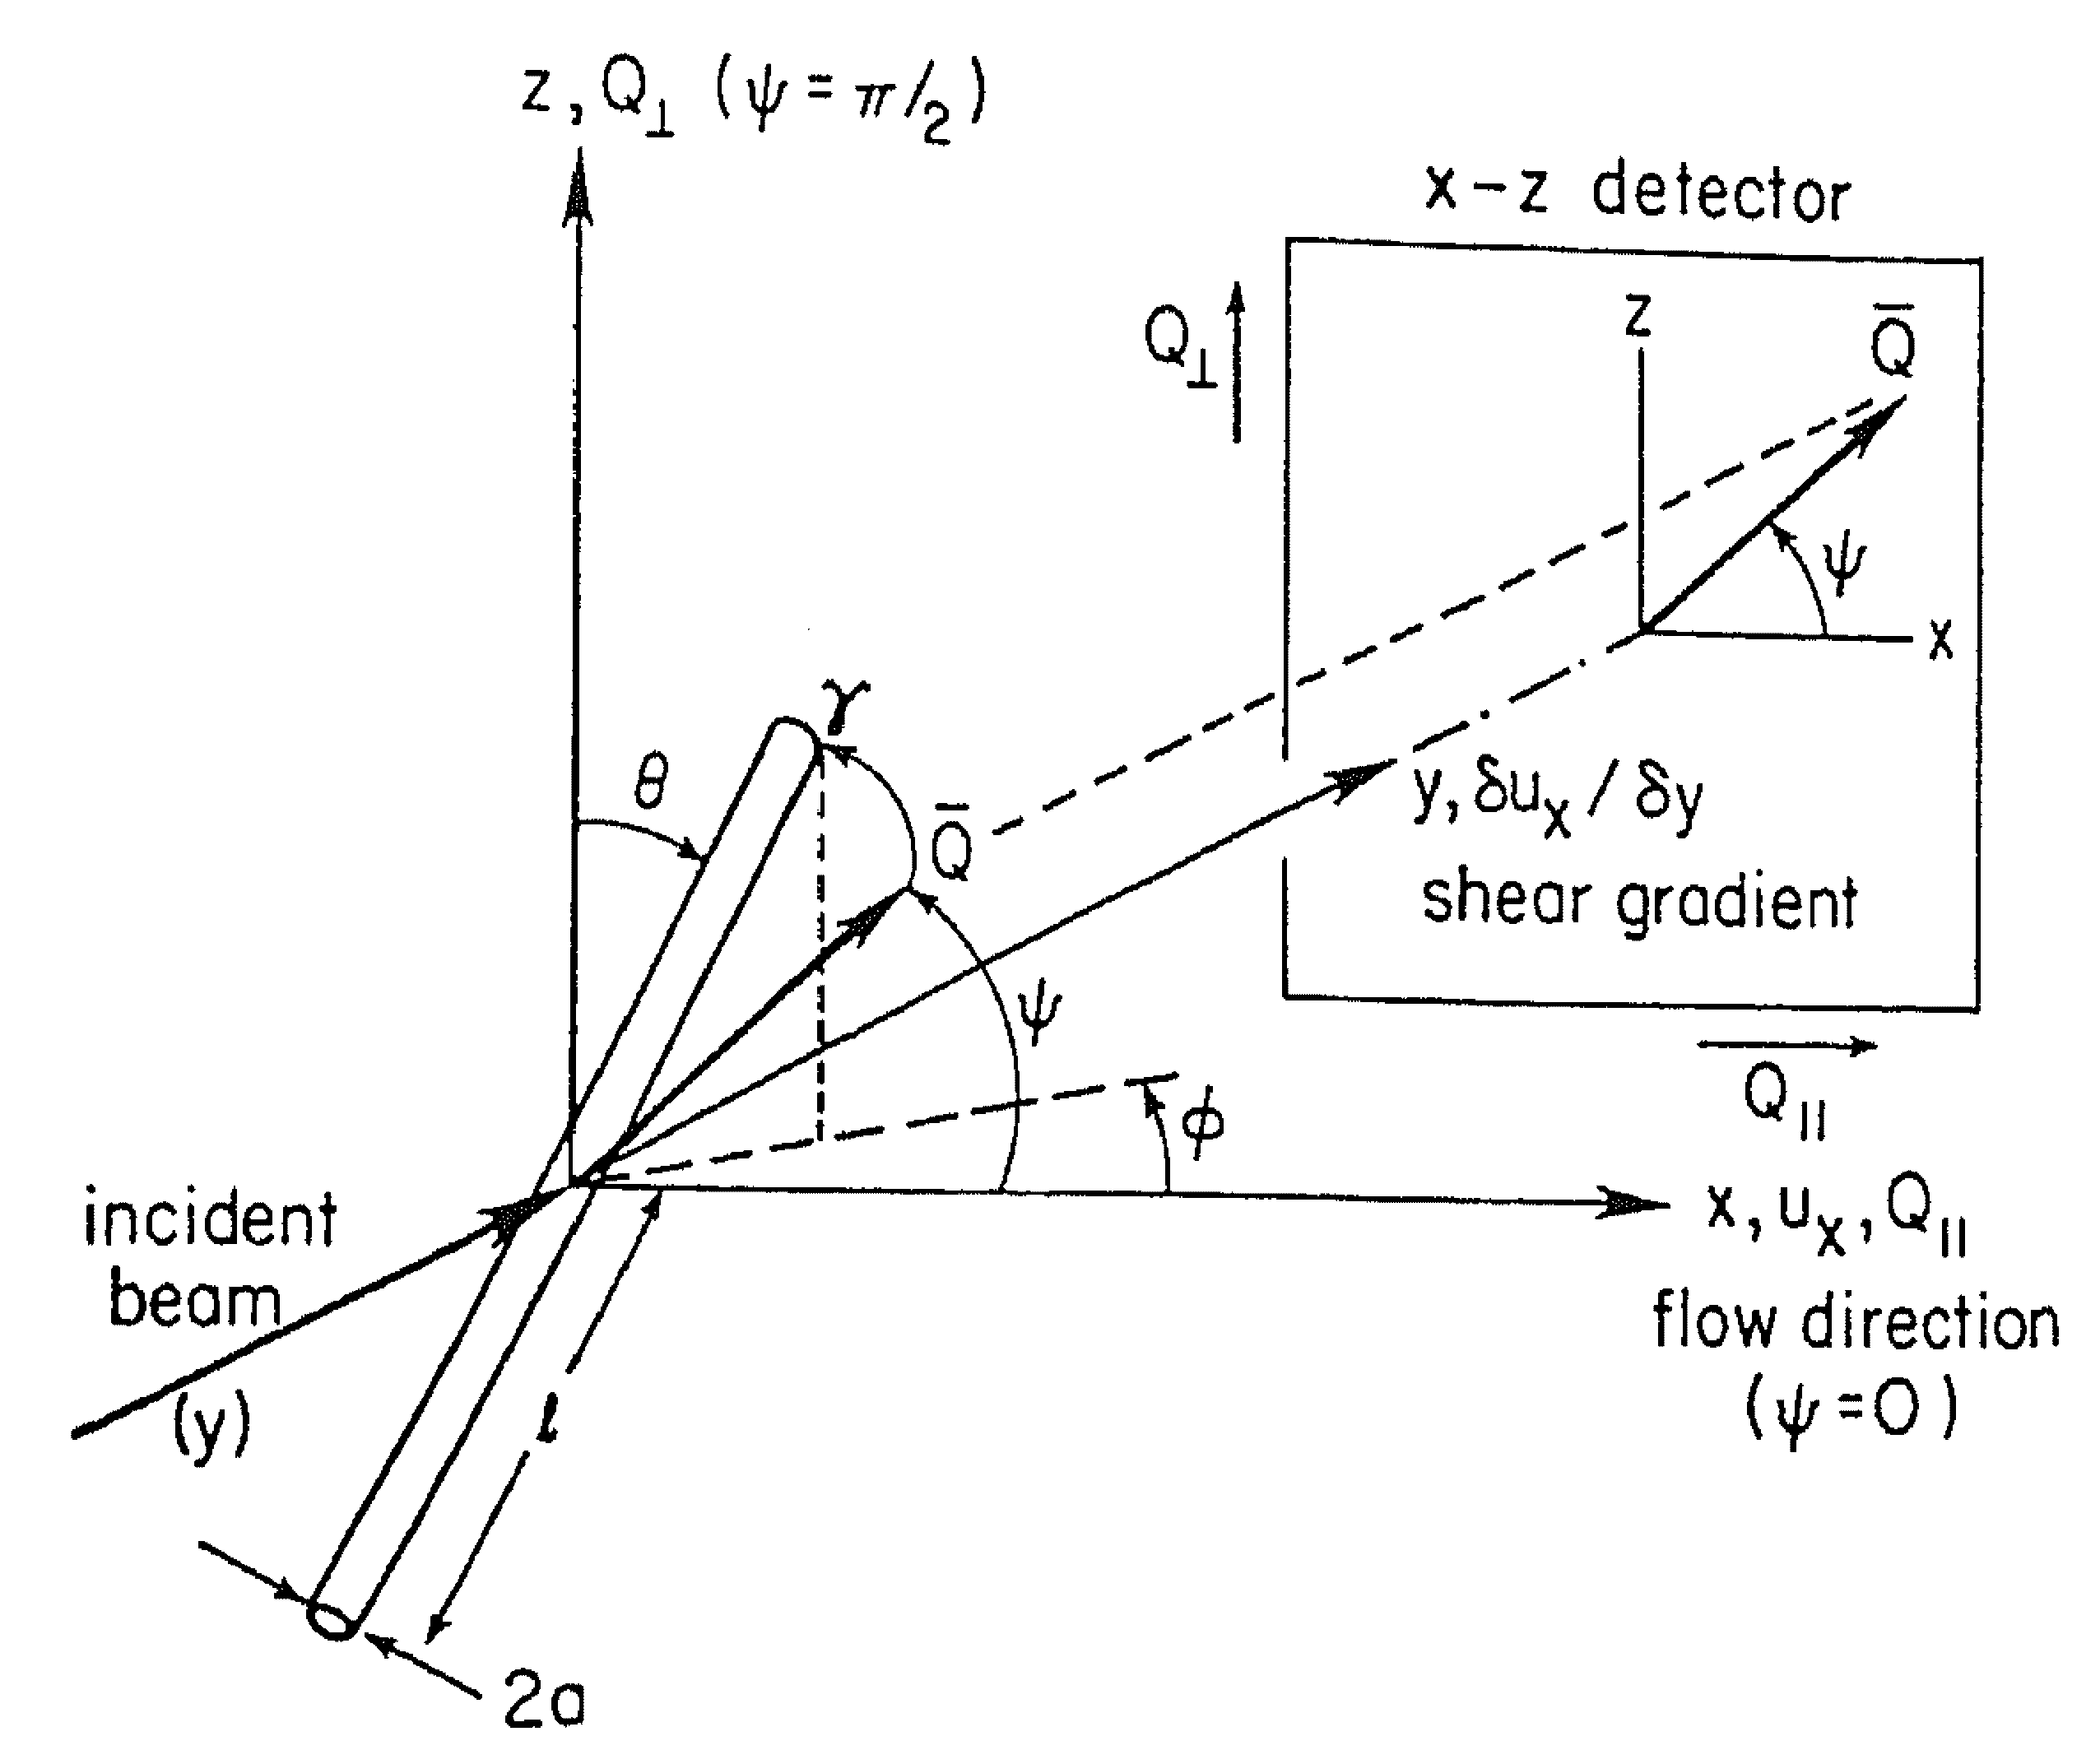
\includegraphics[width=0.7\textwidth]{shear_cuette_SANS_geometry.png}
\end{center}
\caption{Cartesian and angular coordinates referred to the center
of a cylindrical micelle at origin. The relationship to the
spectrometer geometry is shown schematically. The momentum
transfer, $Q$, lies in the $z-x$ plane.}
\label{shear_cuette_SANS_geometry}
\end{figure}

The scattering from monodisperse dilute (non-interacting)
isotropic solution of anisotropic micelles is given by \BE I(Q) =
\left< \vert F(Q)\vert^2 \right>_Q \label{IQ_av} \EE where $F(Q)$
is the form factor for a micelle at a given orientation relative
to the momentum transfer $Q$ and $\left<\right>_Q$ denotes an
average over all such orientations.

For a uniform cylinder of length $L$ and diameter $2R$ the form
factor is given by:
\BE F(Q) = F(Q,\gamma) = 2\Delta\eta V
\frac{\sin\left(QL/2\cos\gamma\right)}{QL/2\cos\gamma}
\frac{J_1(QR\sin\gamma)}{QR\sin\gamma}
\EE
where $\gamma$ is the
angle between $Q$ and the cylinder axis, $V$ is the volume,
$\Delta\eta$ the scattering length density contrast relative to
the solvent, $J_1(x)$ is the first order Bessel function of the
first kind.

The scattering geometry for shear alignment is shown in Fig.
\ref{shear_cuette_SANS_geometry}. In general perfect alignment
will not be achieved, and an orientation distribution must be
employed such that the resultant scattering will be given by
\BE
I(Q,\psi) = \int_0^{2\pi}d\varPhi \int_0^\pi
p(\theta,\varPhi;\Gamma)\, \left(F^2(Q,\gamma^+)+F^2(Q,\gamma^-)
\right) \sin\theta d\theta
\EE
where
\begin{align}
\cos\gamma^\pm & = \sin\theta\cos\phi\cos\psi\pm\cos\theta\sin\psi \\[3mm]
p(\theta,\phi;\Gamma) & = \frac{(1-\cos
2\varPhi_0)(1+\sin^2\theta\cos 2\varPhi_0)^{3/2}}{4\pi\left[
1-\sin^2\theta\cos 2\varPhi_0\cos 2(\phi-\varPhi_0)\right]^2}
\end{align}
and
\BE
2\varPhi_0 = \arctan(8/\Gamma)
\EE
\begin{align}
\frac{\mathbf{Q}}{\abs{\mathbf{Q}}} &=
\begin{pmatrix}
\cos \psi \\
0  \\
\sin \psi
\end{pmatrix} \qquad
\frac{\mathbf{n}}{\abs{\mathbf{n}}} =
\begin{pmatrix}
\sin \theta \cos \phi \\
\sin \theta \sin \phi  \\
\cos \theta
\end{pmatrix} \\
\cos \angle(\mathbf{Q,n}) &= \cos \gamma = \frac{\mathbf{Q\cdot n}}{\abs{\mathbf{Q}}\abs{\mathbf{n}}} =  \cos\psi \sin\theta \cos\phi + \sin\psi \cos\theta
\end{align}

%%%%%%%%%%%%%%%%%%%%%%%%%%%%%%%%%%%%%%%%%%%%%%%%%%%%%%%%%%%%%%%%%%%%%%%%%%%%%%%%%%

\newpage
\subsection{Maier-Saupe orientation distribution} ~\\

\begin{align}
p(\theta,\phi;\kappa) & = \frac{1}{c_\mathrm{MS}}\exp\left(\kappa \cos^2\theta\right) 
\end{align}
with
\begin{align}
c_\mathrm{MS} &=
\begin{cases} 
\displaystyle
4\pi\exp(\kappa) \frac{\mathrm{D}\left(\sqrt{\kappa}\right)}{\sqrt{\kappa}}   &\mathrm{for~} \kappa > 0 \\[5mm]
\displaystyle
2\pi \sqrt{\pi} \frac{\mathrm{erf}\left(\sqrt{\abs{\kappa}}\right)}{\sqrt{\abs{\kappa}}}  &\mathrm{for~} \kappa < 0 \\[2mm]
\displaystyle
4\pi                                                                                      &\mathrm{for~} \kappa = 0
\end{cases}
\end{align}
with $D(x)$ being Dawson's integral $D(x)=e^{-x^2}\int_0^x e^{y^2} \mathrm{d}y = \frac12\sqrt{\pi}e^{-x^2}\mathrm{erfi}(x)$
%%%%%%%%%%%%%%%%%%%%%%%%%%%%%%%%%%%%%%%%%%%%%%%%%%%%%%%%%%%%%%%%%%%%%%%%%%%%%%%%%%

\newpage
\subsection{Onsager orientation distribution} ~\\

\begin{align}
p(\theta,\phi;\kappa) & = 
\begin{cases} \displaystyle
\frac{\kappa \cosh\left(\kappa \cos(\theta)\right)}{4\pi \sinh(\kappa)}      &\mathrm{for~} \kappa \geq 0 \\[5mm]
 \displaystyle
\frac{\cosh\left(\abs{\kappa} sin(\theta)\right)}{2\pi^2 L_1(\abs{\kappa})}  &\mathrm{for~} \kappa < 0 
\end{cases}
\end{align}
where $L_\nu(x)$ is the modified Struve function.

%%%%%%%%%%%%%%%%%%%%%%%%%%%%%%%%%%%%%%%%%%%%%%%%%%%%%%%%%%%%%%%%%%%%%%%%%%%%%%%%%%

\newpage
\subsection{Boltzmann orientation distribution} ~\\

\begin{align}
p(\theta,\phi;\kappa) & = 
\begin{cases}
\displaystyle
\frac{1}{c_\mathrm{B}}\exp\left(-\theta\kappa\right) & \mathrm{for~}  \theta \leq \pi/2\\[5mm]
\displaystyle
\frac{1}{c_\mathrm{B}}\exp\left(-(\pi-\theta)\kappa\right) & \mathrm{for~}  \theta > \pi/2
\end{cases}
\end{align}
with
\begin{align}
c_\mathrm{B} &= \frac{4\pi\left(1-\kappa*exp\left(-\frac{\pi}{2}\kappa\right)\right)}{\kappa^2+1}
\end{align}
%%%%%%%%%%%%%%%%%%%%%%%%%%%%%%%%%%%%%%%%%%%%%%%%%%%%%%%%%%%%%%%%%%%%%%%%%%%%%%%%%%

\newpage
\subsection{Gaussian orientation distribution}
\label{sect:ShearedCylinderGaussian}
~\\
\begin{align}
p(\theta,\phi;\kappa) & = 
\begin{cases}
\displaystyle
\frac{1}{c_\mathrm{G}}\exp\left(-\theta^2\kappa^2\right) & \mathrm{for~} \kappa \geq 0 \mathrm{~and~} \theta \leq \pi/2\\[5mm]
\displaystyle
\frac{1}{c_\mathrm{G}}\exp\left(-(\pi-\theta)^2\kappa^2\right) & \mathrm{for~} \kappa \geq 0 \mathrm{~and~} \theta > \pi/2\\[5mm]
\displaystyle
\frac{1}{c_\mathrm{G}}\exp\left(-(\frac{\pi}{2}-\theta)^2\abs{\kappa}^2\right) & \mathrm{for~} \kappa < 0 
\end{cases}
\end{align}
with
\begin{align}
c_\mathrm{G} & =
\begin{cases}\displaystyle
2\pi\frac{D\left(\kappa/2\right)}{\kappa}
           +2\pi\frac{\sqrt{\pi}}{2\kappa} e^{-\frac{1}{4\kappa^2}} \Re\left(\mathrm{cerfi}\left(-\frac{1}{2\kappa}+\imath\frac{\pi}{2}\kappa\right) \right)& \mathrm{for~} \kappa \geq 0 \\[5mm]
\displaystyle
2\pi\frac{\sqrt{\pi}}{\abs{\kappa}} e^{-\frac{1}{4\kappa^2}} \Im\left(\mathrm{cerfi}\left(-\frac{1}{2\abs{\kappa}}+\imath\frac{\pi}{2}\abs{\kappa}\right) \right) & \mathrm{for~} \kappa < 0
\end{cases}
\end{align}
%%%%%%%%%%%%%%%%%%%%%%%%%%%%%%%%%%%%%%%%%%%%%%%%%%%%%%%%%%%%%%%%%%%%%%%%%%%%%%%%%%

\newpage
\subsection{ShearedCylinderHeaviside} ~\\

\begin{align}
p(\theta,\phi;\bar{\theta}) & = \Theta[\theta-\bar{\theta}] \\
\cos\gamma^\pm & = \sin\theta\cos\phi\cos\psi\pm\cos\theta\sin\psi
\end{align}

%\item[ShearedCylinderMaierSaupe] ~\\
%\begin{align}
%p(\theta,\phi;\bar{\theta}) & = \exp[\cos^2(\theta/\bar{\theta})]-1 \\
%\cos\gamma^\pm              & = \sin\theta \cos\phi \sin\psi \pm \cos\theta\cos\phi
%\end{align}
%
%\item[ShearedCylinderOnsager] ~\\
%\begin{align}
%p(\theta,\phi;\bar{\theta}) & = \exp[-\sin(\theta/\bar{\theta})] \\
%\cos\gamma^\pm              & = \sin\theta \cos\phi \sin\psi \pm \cos\theta\cos\phi
%\end{align}

